\chapter{CMOS Inverter-Based Amplifier}
\label{chap:amplifier}

This chapter details the design, simulation, and verification of a CMOS inverter-based amplifier intended for use in a neural interface application. The amplifier utilizes open-source tools throughout the design workflow, adhering to the SkyWater 130nm CMOS PDK.
\\
This chapter presents only the results for the latest version of the amplifier design. Previous simulation results and designs can be found in Appendix \ref{AppendixB}.
\\
All files related to the amplifier design can be found in \textcite{miguelcorrea0107_2024}.

\section{Design Specifications}

The amplifier design targets the following specifications established for neural interface applications:

\begin{itemize}
\item \textbf{Power Supply Voltage:} 0.5V to 1.5V (Flexibility for various neural recording setups)
\item \textbf{Input-Referred Noise:} Around 3 $\mu$V between 300 Hz to 10 kHz (Minimizes noise contribution to the neural signal)
\item \textbf{Gain:} Around 20 dB (Amplifies weak neural signals)
\item \textbf{Frequency Response:} Bandpass with flat gain between 10 Hz to 5 kHz (Focuses on the relevant frequency range of neural activity)
\item \textbf{Power Consumption:} Less than 10 $\mu$W (Low power consumption for extended device operation)
\item \textbf{Device Size:} Minimized for efficient chip area utilization
\end{itemize}

\section{Design Choices}
The final design of the amplifier is based on several strategic choices to optimize performance and minimize the footprint. 
Transistor fingering was employed to optimize the layout size, ensuring efficient use of the available area. 
Active resistors were chosen for their ability to provide high gain and low noise while maintaining a small footprint. 
Additionally, transistor-based capacitors were utilized to further reduce the overall footprint of the design. 
These design choices collectively contribute to achieving the desired specifications for the neural interface application.

\section{Schematic Design}
The amplifier design leverages a inverter architecture inspired by the work presented in \textcite{Yuan_Hierlemann_Frey_2021}.
Employing Xschem and the SkyWater 130nm PDK libraries, the schematic diagram and symbol for the circuit were created. 
Figure \ref{fig:schematic_v4} shows the schematic diagram of the amplifier design.

\begin{figure}[ht!]
\centering
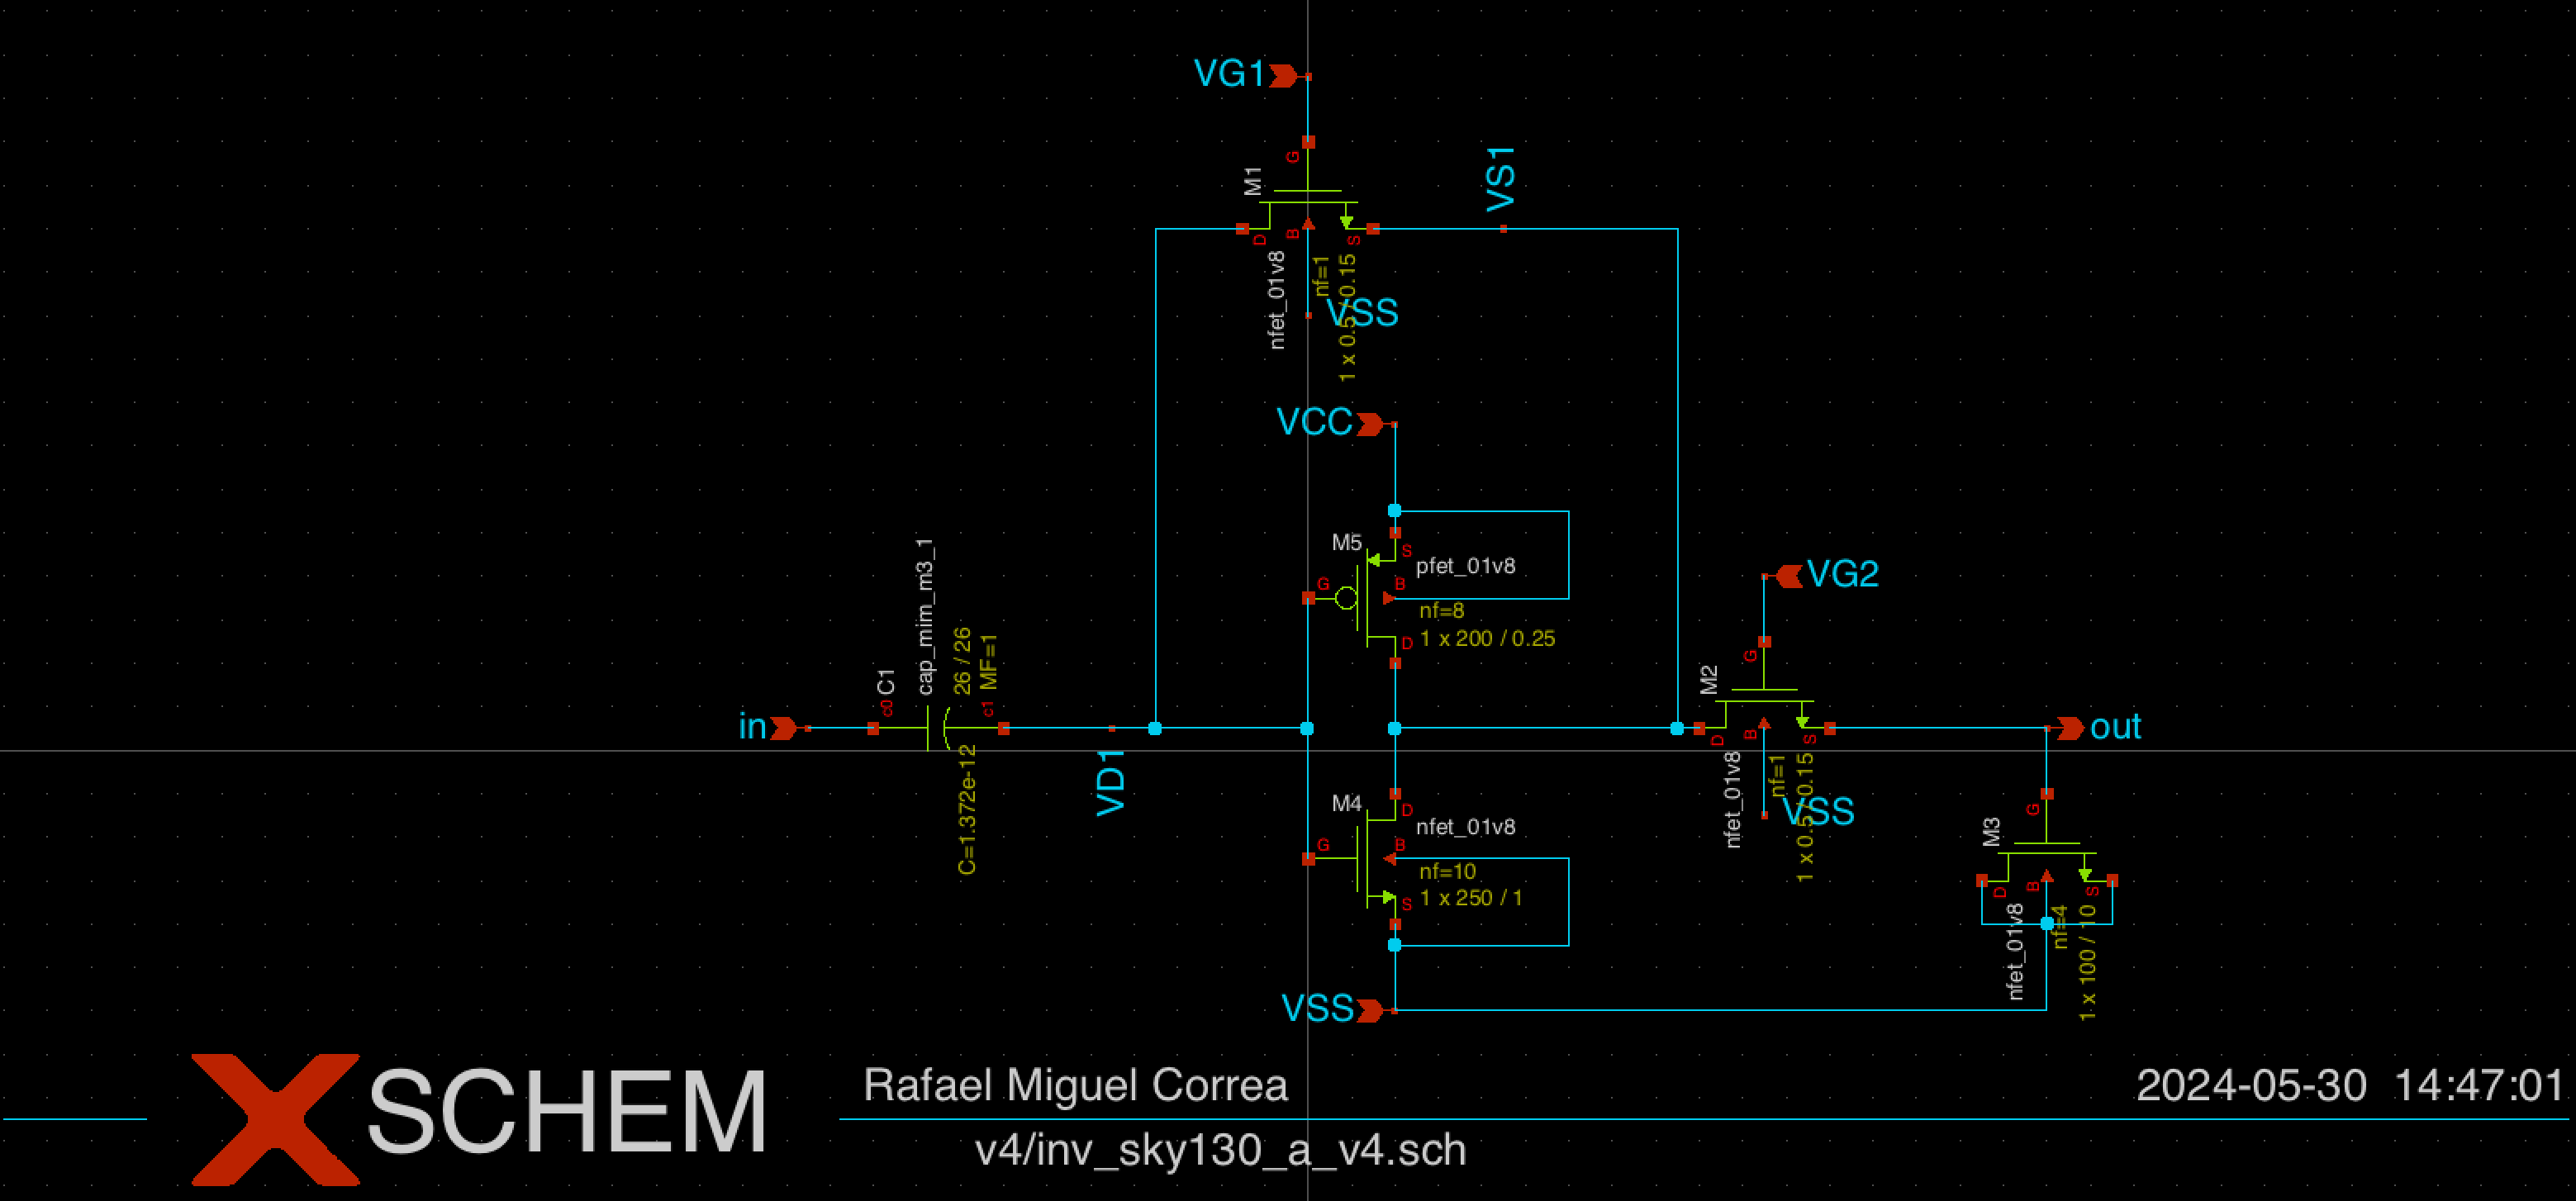
\includegraphics[width=\textwidth]{Figures/v4_schematic.png}
\caption{Schematic diagram of the CMOS inverter-based amplifier design.}
\label{fig:schematic_v4}
\end{figure}

\section{Simulation Results}

SPICE simulations were conducted using ngspice on a testbench (see Figure \ref{fig:testbench_v4}) to assess the amplifier's performance under various conditions. 
A test bench was designed in Xschem to automate a series of simulations, including:

\begin{itemize}
\item \textbf{Operating Point Analysis:} Determines the stable biasing condition for the transistors.
\item \textbf{AC Response:} Evaluates the amplifier's gain and frequency response (see Figure \ref{fig:frequency_response_v4}).
\item \textbf{Noise Analysis:} Estimates the input-referred noise of the amplifier (see Figure \ref{fig:noise_v4}).
\item \textbf{Transient Simulation:} Calculates the average power consumption of the amplifier during operation.
\item \textbf{DC Characteristic:} Sweeps the input voltage and measures the output voltage to determine the transfer function.
\item \textbf{Corner Simulation:} Simulates the amplifier under process, voltage, and temperature variations.
\end{itemize}

Unfortunately, Monte Carlo simulations were not performed due to time constraints and because the PDK did not provide the necessary information for the simulations.

Corner simulations showed changes in the frequency response and noise values. To address this issue, post-fabrication tuning of the amplifier will be necessary. 
Specifically, adjusting the values of $V_{g1}$ and $V_{g2}$ will ensure the amplifier meets the desired specifications.

The simulation results are as follows:

\begin{itemize}
\item \textbf{Gain:} 20.89885 dB
\item \textbf{Bandwidth:} 8.87156 Hz to 4.375 kHz
\item \textbf{Noise:} 5.751697 $\mu$V between 300 Hz to 10 kHz
\item \textbf{Power Consumption:} 3.115 $\mu$W
\end{itemize}

\begin{figure}[ht!]
\centering
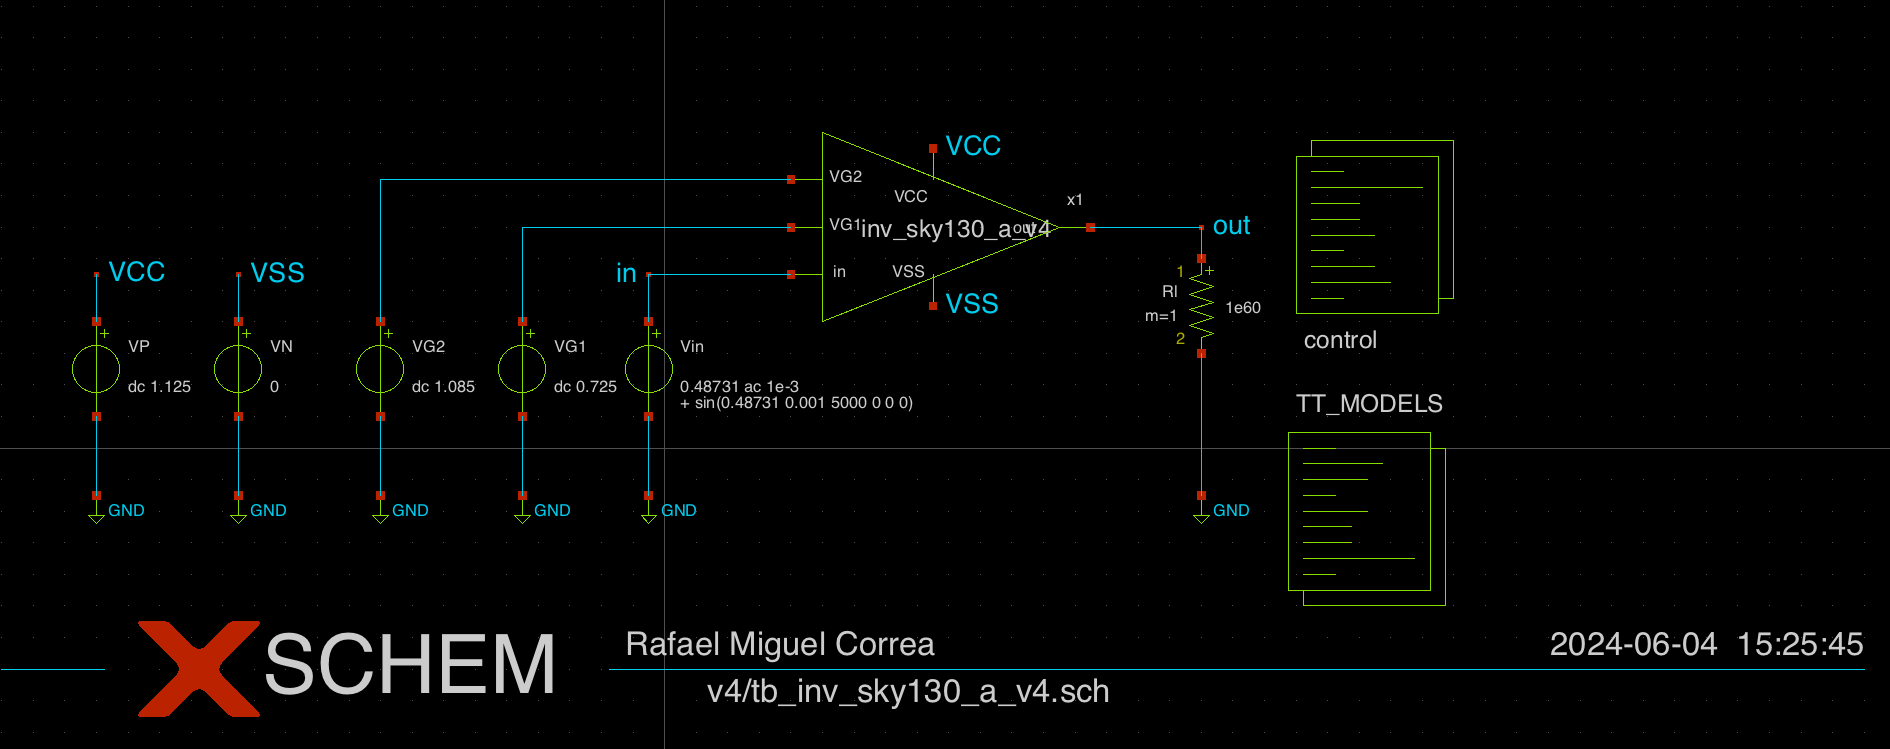
\includegraphics[width=\textwidth]{Figures/testbench.png}
\caption{Testbench for the CMOS inverter-based amplifier design.}
\label{fig:testbench_v4}
\end{figure}

\begin{figure}[ht!]
\centering
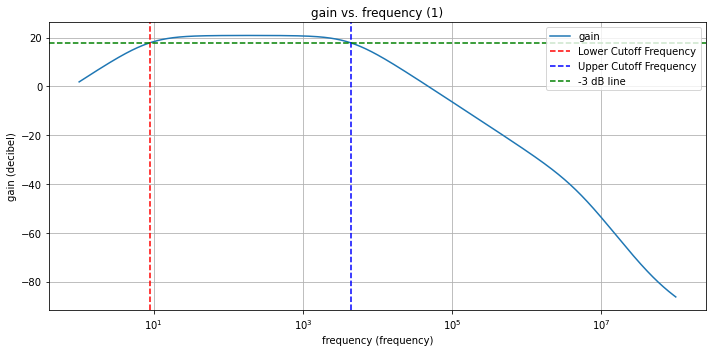
\includegraphics[width=\textwidth]{Figures/frequency_response_v4.png}
\caption{Frequency response of the CMOS inverter-based amplifier design.}
\label{fig:frequency_response_v4}
\end{figure}

\begin{figure}[ht!]
\centering
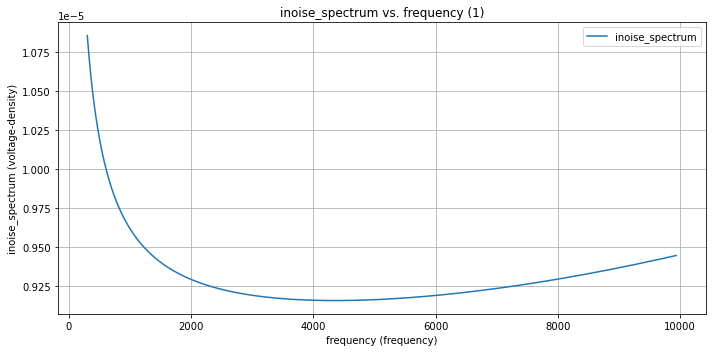
\includegraphics[width=\textwidth]{Figures/v4_noise_sim_results.png}
\caption{Noise analysis of the CMOS inverter-based amplifier design.}
\label{fig:noise_v4}
\end{figure}

\section{Layout Design}

Magic was used to translate the schematic design into a manufacturable layout. 
Figure \ref{fig:layout_v4} shows the layout design of the CMOS inverter-based amplifier. This layout results in:

\begin{itemize}
\item \textbf{Width:} 27.4 $\mu$m
\item \textbf{Height:} 67.95 $\mu$m
\item \textbf{Total Area:} 1861.83 $\mu$m$^2$
\end{itemize}

The layout is designed to minimize unused space and ensure efficient use of the available area.

\begin{figure}[ht!]
\centering
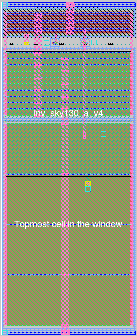
\includegraphics[width=0.6\textwidth]{Figures/final_layout.png}
\caption{Layout design of the CMOS inverter-based amplifier.}
\label{fig:layout_v4}
\end{figure}

The layout design was subjected to a rigorous DRC using Magic to ensure adherence to the SkyWater 130nm CMOS PDK foundry rules. 
This step guarantees the manufacturability of the designed layout.

Following a successful DRC check, a LVS verification was performed using Netgen. 
This process confirms that the physical layout accurately reflects the intended electrical connectivity of the schematic.

\section{Post-Layout Simulation}
Post-layout simulations were conducted using the extracted parasitic information to obtain a more realistic prediction of the amplifier's performance after fabrication. 
Table \ref{tab:specifications_comp} summarizes the post-layout simulation specifications in comparison to the desired specifications.
\\
Additionnaly, figure \ref{fig:post_layout_frequency_response} shows the frequency response of the CMOS inverter-based amplifier design post-layout, 
and figure \ref{fig:post_layout_noise} shows the noise analysis of the CMOS inverter-based amplifier design after post-layout.

\begin{table}[ht!]
    \centering
    \resizebox{\textwidth}{!}{
    \begin{tabular}{|l|c|c|}
    \hline
    \textbf{Specification} & \textbf{Desired Value} & \textbf{Final Value} \\ \hline
    Power Supply Voltage & 0.5V to 1.5V & 1.125V \\ \hline
    Input-Referred Noise & Around 3 $\mu$V between 300 Hz to 10 kHz & 5.997 $\mu$V between 300 Hz to 10 kHz \\ \hline
    Gain & Around 20 dB & 19.056 dB \\hline
    Frequency Response & Bandpass, 10 Hz to 5 kHz & Bandpass, 6.887 Hz to 4.688 kHz \\ \hline
    Power Consumption & Less than 10 $\mu$W & 3.163 $\mu$W \\ \hline
    Device Size & - & 1861.83 $\mu$m$^2$ \\ \hline
    \end{tabular}
    }
    \caption{Specification Comparison}
    \label{tab:specifications_comp}
\end{table}

\begin{figure}[ht!]
    \centering
    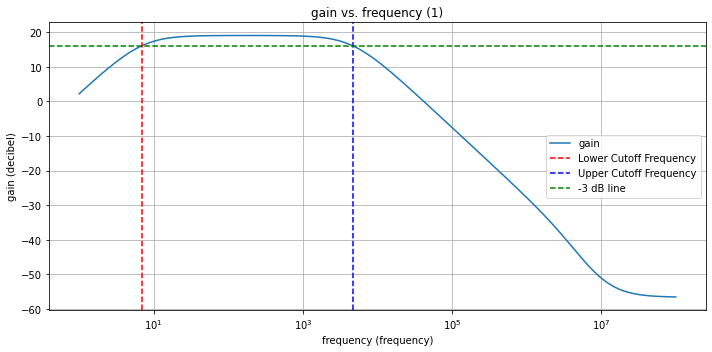
\includegraphics[width=\textwidth]{Figures/post_layout_frequency_response.png}
    \caption{Frequency response of the CMOS inverter-based amplifier design after layout.}
    \label{fig:post_layout_frequency_response}
\end{figure}

\begin{figure}[ht!]
    \centering
    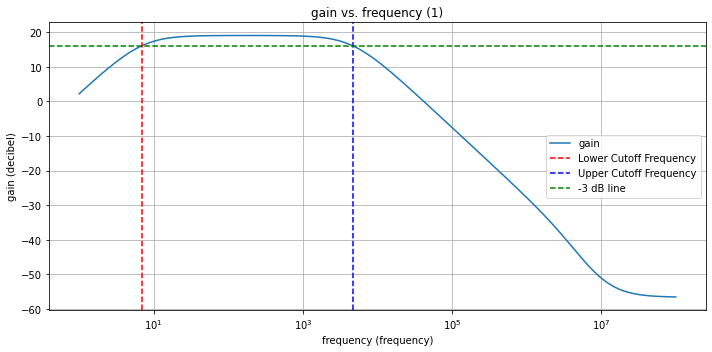
\includegraphics[width=\textwidth]{Figures/post_layout_frequency_response.png}
    \caption{Noise analysis of the CMOS inverter-based amplifier design after layout.}
    \label{fig:post_layout_noise}
\end{figure}

\section{Conclusion}
The post-layout simulation results show that the amplifier meets most of the desired specifications, with slight deviations in the gain and noise levels. 
The power consumption is well within the desired range, and the frequency response, while slightly narrower, still falls within an acceptable range. 
These results indicate that the design is robust and manufacturable, with only minor adjustments needed to optimize performance further. 
The successful completion of DRC, LVS, and post-layout simulations demonstrates the readiness of the CMOS inverter-based amplifier project for fabrication, though adjustments for process variations were identified as necessary. 